\documentclass[utf8,compress]{beamer}
\usepackage{irbookslide}
\usepackage{irilmenau2}
\usepackage{url}
\usepackage{fontspec} % zahteva paket euenc
\usepackage{xunicode}
\usepackage{xltxtra}
\usepackage{polyglossia}
\usepackage[cache=false]{minted}
\usepackage{xcolor,colortbl}
\usepackage{textcomp}
\usepackage{unicode-math}

\title{Grananje u programu}
\subtitle{\tiny{Slajdovi za predmet Osnove programiranja}}
\subject{Osnove programiranja}
\institute{Katedra za informatiku, Fakultet tehničkih nauka, Novi Sad}
\date{2017.}

\begin{document}

% da pygmentize ne uokviruje crvenom bojom nepoznate karaktere
\expandafter\def\csname PY@tok@err\endcsname{}

\frame{\titlepage}

\frame{
  \frametitle{Ciljevi}
  \begin{itemize}
    \item razumevanje grananja u programu i Pythonove \texttt{if} naredbe
    \item dvostruko grananje i \texttt{if-else} naredba
    \item višestruko grananje i \texttt{if-elif-else} naredba
    \item pojam obrade izuzetaka (exceptions)
    \item pisanje koda za obradu izuzetaka
  \end{itemize}
}

\frame{
  \frametitle{Ciljevi}
  \begin{itemize}
    \item Bulovi izrazi i \texttt{bool} tip podataka
    \item kreiranje algoritama koji uključuju elemente kontrole toka
    \item uključujući nizove grananja i ugnježdeno grananje
  \end{itemize}
}

\section{1-grananje}

\frame{
  \frametitle{Jednostavno grananje}
  \begin{itemize}
    \item do sada smo videli programe koji predstavljaju proste sekvence instrukcija koje slede jedna drugu
    \item to nam nije dovoljno za rešavanje svih problema
    \item nekada je potrebno izmeniti tok instrukcija da bismo rešili problem
  \end{itemize}
}

\begin{frame}[fragile]
  \frametitle{Primer: temperatura}
  \begin{itemize}
    \item podsetimo se primera za konverziju temperature $^o$C $\rightarrow$ $^o$F
  \end{itemize}
\begin{minted}[linenos=false]{python}
# convert.py

def main():
    celsius = eval(raw_input("Unesite temperaturu C >> "))
    fahrenheit = 9.0/5 * celsius + 32
    print "Temperatura je ", fahrenheit, 
        "stepeni Farenhajta."

main()
\end{minted}
\end{frame}

\frame{
  \frametitle{Primer: temperatura $_2$}
  \begin{itemize}
    \item sada treba izmeniti program tako da ispiše upozorenje za ekstremne vrednosti temperature
    \item temperatura iznad $90^o$F ili ispod $30^o$F će biti ekstremna
  \end{itemize}
}

\frame{
  \frametitle{Primer: temperatura $_3$}
  \begin{itemize}
    \item[1] unesi temperaturu u $^o$C
    \item[2] izračunaj temperaturu u $^o$F
    \item[3] ispiši temperaturu u $^o$F
    \item[4] ako je $f \geq 90$ \\
      \ \ \ \ ispiši upozorenje o visokoj temperaturi
    \item[5] ako je $f \leq 30$ \\
      \ \ \ \ ispiši upozorenje o niskoj temperaturi
  \end{itemize}
}

\frame{
  \frametitle{Primer: temperatura $_4$}
  \begin{itemize}
    \item ovaj algoritam ima dva grananja na kraju
    \item uvlačenje teksta sugeriše da se dati korak treba izvršiti samo u slučaju da je ispunjen uslov iz prethodnog reda
  \end{itemize}
}

\frame{
  \frametitle{Primer: temperatura $_5$}
  \begin{center}
    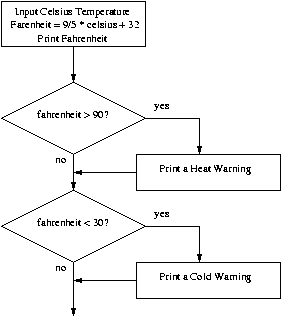
\includegraphics[width=6cm]{pic13}
  \end{center}
}

\begin{frame}[fragile]
  \frametitle{Primer: temperatura $_6$}
\begin{minted}[linenos=false]{python}
# convert2.py

def main():
    c = eval(raw_input("Unesite temperaturu u C: "))
    f = 9.0 / 5 * c + 32
    print "Temperatura je", f, "stepeni Farenhajta."
    if f >= 90:
        print "Baš je vrućina!"
    if f <= 30:
        print "Brrrrr. Dobro se obuci!"

main()
\end{minted}
\end{frame}

\frame{
  \frametitle{Naredba \texttt{if}}
  \begin{itemize}
    \item naredba \texttt{if} služi za implementaciju grananja
    \item \texttt{if <uslov>:} \\
      \texttt{\ \ \ \ <telo>}
    \item \texttt{telo} je niz naredbi koje su uvučene u odnosu na \texttt{if} izraz
  \end{itemize}
}

\frame{
  \frametitle{Izvršavanje \texttt{if} naredbe}
  \begin{itemize}
    \item prvo se izračuna uslov
    \item ako je uslov \myblue{ispunjen}, niz naredbi u telu se \myblue{izvršava}, i program se dalje izvršava nakon \texttt{if} naredbe
    \item ako uslov \myblue{nije ispunjen}, niz naredbi u telu se \myblue{preskače}, i program se izvršava nakon \texttt{if} naredbe
  \end{itemize}
}

\frame{
  \frametitle{Izvršavanje \texttt{if} naredbe $_2$}
  \begin{center}
    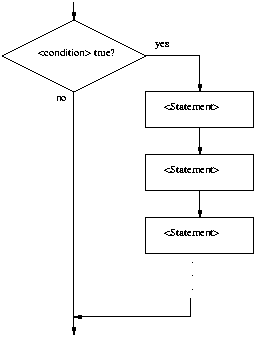
\includegraphics[width=5cm]{pic14}
  \end{center}
}

\frame{
  \frametitle{Izvršavanje \texttt{if} naredbe $_3$}
  \begin{itemize}
    \item telo \texttt{if} naredbe izvršava se ili se ne izvršava u zavisnosti od uslova
    \item u svakom slučaju izvršavanje se nastavlja od naredbe koja sledi posle \texttt{if}
    \item ovo je jednostavno ili \myblue{jednostruko} grananje
  \end{itemize}
}

\section{Poređenje}

\frame{
  \frametitle{Pisanje uslova za \texttt{if}}
  \begin{itemize}
    \item za početak, pišemo jednostavne izraze poređenja
    \item \texttt{<izraz> <relop> <izraz>}
    \item \texttt{relop} je oznaka za relacioni operator
  \end{itemize}
  \begin{center}
    \begin{tabular}{c|c|l}
      \textbf{python} & \textbf{matematika} & \textbf{značenje} \\ \hline
      \texttt{<} & $<$ & manje od \\ \hline
      \texttt{<=} & $\leq$ & manje ili jednako \\ \hline
      \texttt{==} & $=$ & jednako \\ \hline
      \texttt{>=} & $\geq$ & veće ili jednako \\ \hline
      \texttt{>} & $>$ & veće od \\ \hline
      \texttt{!=} & $\neq$ & nije jednako
    \end{tabular}
  \end{center}
}

\frame{
  \frametitle{\texttt{=} i \texttt{==}}
  \begin{itemize}
    \item za poređenje koristi se \texttt{==} umesto \texttt{=}
    \item znak \texttt{=} je rezervisan za operaciju dodele vrednosti
    \item uobičajena greška je da pišemo \texttt{=} prilikom poređenja
  \end{itemize}
}

\frame{
  \frametitle{Poređenje stringova}
  \begin{itemize}
    \item možemo porediti brojeve i stringove
    \item kada poredimo stringove, koristi se \myblue{leksikografski} redosled
    \item tj. stringovi se sortiraju prema Unicode kodovima znakova
    \begin{itemize}
      \item velika slova su ,,manja`` od malih, dakle \\ 
        \texttt{"Bbbb" < "aaaa"}
    \end{itemize}
  \end{itemize}
}

\frame{
  \frametitle{Bulovi izrazi}
  \begin{itemize}
    \item uslov je Bulov izraz (George Boole 1815-1864)
    \item Bulov izraz može imati samo dve vrednosti, 
    \begin{itemize}
      \item \myblue{tačno} (uslov je ispunjen)
      \item \myblue{netačno} (uslov nije ispunjen)
    \end{itemize}
    \item Python ima konstante \texttt{True} i \texttt{False}
    \item u nekim jezicima 0 označava netačno, a 1 tačno
  \end{itemize}
}

\begin{frame}[fragile]
  \frametitle{Bulovi izrazi $_2$}
  \begin{itemize}
    \item Bulovi izrazi su tipa \texttt{bool} 
    \item dve moguće vrednosti: \texttt{True} i \texttt{False}
  \end{itemize}
\begin{verbatim}
>>> 3 < 4
True
>>> 3 * 4 < 3 + 4
False
>>> "hello" == "hello"
True
>>> "Hello" < "hello"
True
\end{verbatim}
\end{frame}

\section{2-grananje}

\begin{frame}[fragile]
  \frametitle{Primer: kvadratna jednačina}
  \begin{itemize}
    \item podsetimo se programa za rešavanje kvadratne jednačine
  \end{itemize}
\begin{minted}[linenos=false]{python}
import math

def main():
    a, b, c = eval(raw_input(
        "Unesite koeficijente (a, b, c): "))
    discRoot = math.sqrt(b * b - 4 * a * c)
    root1 = (-b + discRoot) / (2 * a)
    root2 = (-b - discRoot) / (2 * a)
    print "\nRešenja su:", root1, root2

main()
\end{minted}
\end{frame}

\begin{frame}[fragile]
  \frametitle{Primer: kvadratna jednačina $_2$}
  \begin{itemize}
    \item ako je $b^2 - 4ac < 0$, program će pući
  \end{itemize}
\begin{verbatim}
Unesite koeficijente (a, b, c): 1,1,2

Traceback (most recent call last):
  File "/home/branko/pajton/quadratic.py", line 13, in -toplevel-
    main()
  File "/home/branko/pajton/quadratic.py", line 8, in main
    discRoot = math.sqrt(b * b - 4 * a * c)
ValueError: math domain error
\end{verbatim}
\end{frame}

\begin{frame}[fragile]
  \frametitle{Primer: kvadratna jednačina $_3$}
  \begin{itemize}
    \item možemo da proverimo ovaj uslov; prvi pokušaj:
  \end{itemize}
\begin{minted}[linenos=false]{python}
# quadratic2.py
import math  

def main():
    a, b, c = eval(raw_input(
        "Unesite koeficijente (a, b, c): "))

    discrim = b * b - 4 * a * c
    if discrim >= 0:
        discRoot = math.sqrt(discrim)
        root1 = (-b + discRoot) / (2 * a)
        root2 = (-b - discRoot) / (2 * a)
        print "\nRešenja su:", root1, root2
\end{minted}
\end{frame}

\begin{frame}[fragile]
  \frametitle{Primer: kvadratna jednačina $_4$}
  \begin{itemize}
    \item prvo računamo diskriminantu $b^2-4ac$ i proveravamo da li je nenegativna
    \item ako jeste, program nastavlja sa telom if naredbe i izračunavamo koren
    \item u suprotnom slučaju program se završava ne ispisujući nikakvu poruku!
    \item skoro da je ovo lošije nego prethodna greška, jer korisnik nema obaveštenje o tome šta se desilo
  \end{itemize}
\end{frame}

\begin{frame}[fragile]
  \frametitle{Primer: kvadratna jednačina $_5$}
  \begin{itemize}
    \item mogli bismo dodati još jedan \texttt{if} na kraj programa: \\
        \texttt{if discrim < 0:} \\
        \texttt{\ \ \ \ print "Nema realnih korena!"}
    \item ovo će raditi ali nije elegantno
    \item imamo dva uslova koji su \myblue{međusobno isključiva}
  \end{itemize}
\end{frame}

\begin{frame}[fragile]
  \frametitle{Dvostruko grananje}
  \begin{center}
    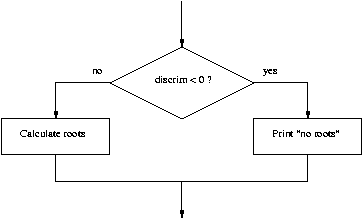
\includegraphics[width=9cm]{pic15}
  \end{center}
\end{frame}

\begin{frame}[fragile]
  \frametitle{Dvostruko grananje $_2$}
  \begin{itemize}
    \item u Pythonu možemo napraviti dvostruko grananje dodavanjem \texttt{else} klauzule na kraj \texttt{if} klauzule
    \item ovo se zove \texttt{if-else} naredba: \\
        \texttt{if <uslov>:} \\
        \texttt{\ \ \ \ <naredbe>} \\
        \texttt{else:} \\
        \texttt{\ \ \ \ <naredbe>}
  \end{itemize}
\end{frame}

\begin{frame}[fragile]
  \frametitle{Dvostruko grananje $_3$}
  \begin{itemize}
    \item kada Pyhon naiđe na \texttt{if-else} naredbu
    \item prvo se izračunava uslov
    \item ako je uslov \myblue{ispunjen}, izvršavaju se naredbe ispod \texttt{if}
    \item ako uslov \myblue{nije ispunjen}, izvršavaju se naredbe ispod \texttt{else}
    \item u oba slučaja izvršavanje se nastavlja sa naredbama posle \texttt{if-else}
  \end{itemize}
\end{frame}

\begin{frame}[fragile,shrink=5]
  \frametitle{Primer: kvadratna jednačina}
\begin{minted}[linenos=false]{python}
# quadratic3.py
import math 

def main():
    a, b, c = eval(raw_input(
        "Unesite koeficijente (a, b, c): "))
    discrim = b * b - 4 * a * c
    if discrim < 0:
        print "\nNema realnih korena!"
    else:
        discRoot = math.sqrt(b * b - 4 * a * c)
        root1 = (-b + discRoot) / (2 * a)
        root2 = (-b - discRoot) / (2 * a)
        print "\nRešenja su:", root1, root2

main()
\end{minted}
\end{frame}

\begin{frame}[fragile]
  \frametitle{Primer: kvadratna jednačina $_2$}
\begin{verbatim}
>>> 
Unesite koeficijente (a, b, c): 1,1,2

Nema realnih korena!

>>> 
Unesite koeficijente (a, b, c): 2, 5, 2

Rešenja su: -0.5 -2.0
\end{verbatim}
\end{frame}

\section{n-grananje}

\begin{frame}[fragile]
  \frametitle{Višestruko grananje}
  \begin{itemize}
    \item poslednji program i dalje ima problema!
  \end{itemize}
\begin{verbatim}
Unesite koeficijente (a, b, c): 1,2,1

Rešenja su: -1.0 -1.0
\end{verbatim}
\end{frame}

\begin{frame}[fragile]
  \frametitle{Višestruko grananje $_2$}
  \begin{itemize}
    \item program radi ispravno, ali može da zbuni korisnika -- izgleda kao da je greškom dva puta ispisao istu vrednost
    \item dva ista korena dobijaju se kada je diskriminanta jednaka 0
    \item tada koren ima vrednost $-b/2a$
    \item treba nam trostruko grananje!
  \end{itemize}
\end{frame}

\begin{frame}[fragile]
  \frametitle{Višestruko grananje $_3$}
\begin{verbatim}
izračunaj vrednost diskriminante
   kada je < 0: slučaj kad nema realnih korena
   kada je = 0: slučaj kad ima jedan koren
   kada je > 0: slučaj kad ima dva realna korena
\end{verbatim}
  \begin{itemize}
    \item ovo možemo rešiti sa dva \texttt{if}-a, jedan unutar drugog
    \item umetanje jedne složene naredbe unutar druge zove se \myblue{ugnježdavanje}
  \end{itemize}
\end{frame}

\begin{frame}[fragile]
  \frametitle{Višestruko grananje $_4$}
\begin{minted}[linenos=false]{python}
if discrim < 0:
    print "Nema realnih korena!"
else:
    if discrim == 0:
        root = -b / (2 * a)
        print "Ima jedan koren:", root
    else:
        # odradi dva korena
\end{minted}
\end{frame}

\begin{frame}[fragile]
  \frametitle{Višestruko grananje $_5$}
\begin{center}
  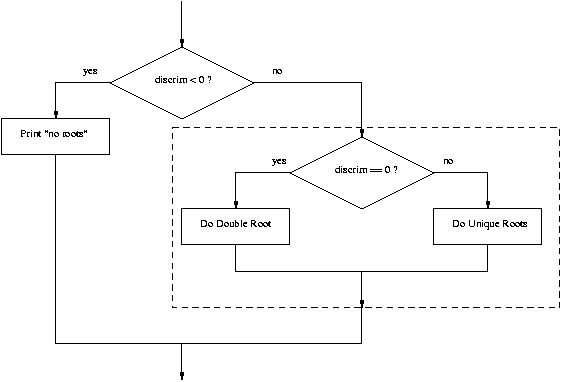
\includegraphics[width=10.5cm]{pic16}
\end{center}
\end{frame}

\begin{frame}[fragile]
  \frametitle{Višestruko grananje $_6$}
  \begin{itemize}
    \item ako nam treba petostruko grananje, imali bismo ugnježdene if-else naredbe na četiri nivoa!
    \item umesto rogobatnog uvlačenja, možemo koristiti \texttt{if-elif-else} naredbu
  \end{itemize}
\begin{minted}[linenos=false]{python}
if <uslov1>:
   <naredbe>
elif <uslov2>:
   <naredbe>
elif <uslov3>:
   <naredbe>
...
else:
   <naredbe>
\end{minted}
\end{frame}

\begin{frame}[fragile]
  \frametitle{Višestruko grananje $_7$}
  \begin{itemize}
    \item samo jedan blok naredbi će biti izvršen
    \item izračunavaju se uslovi, jedan-po-jedan, i traži se prvi koji je \texttt{True}
    \item ako se nađe takav uslov, izvršava se blok naredbi ispod njega
    \item ako se ne nađe, izvršava se blok ispod \texttt{else}
    \item \texttt{else} klauzula nije obavezna!
  \end{itemize}
\end{frame}

\begin{frame}[fragile,shrink=5]
  \frametitle{Višestruko grananje $_8$}
\begin{minted}[linenos=false]{python}
import math 
def main():
    a, b, c = eval(raw_input(
        "Unesite koeficijente (a, b, c): "))
    discrim = b * b - 4 * a * c
    if discrim < 0:
        print "\nNema realnih korena!"
    elif discrim == 0:
        root = -b / (2 * a)
        print "\nIma jedan koren:", root
    else:
        discRoot = math.sqrt(b * b - 4 * a * c)
        root1 = (-b + discRoot) / (2 * a)
        root2 = (-b - discRoot) / (2 * a)
        print "\nRešenja su:", root1, root2
\end{minted}
\end{frame}

\section{Izuzeci}

\begin{frame}[fragile]
  \frametitle{Obrada izuzetaka}
  \begin{itemize}
    \item izbegavali smo grešku u programu (izračunavanje korena negativnog broja) tako što smo koristili grananje
    \item u mnogim slučajevima -- grananje koristimo da se zaštitimo od grešaka
    \begin{itemize}
      \item možda retkih ali ipak mogućih
    \end{itemize}
  \end{itemize}
\end{frame}

\begin{frame}[fragile]
  \frametitle{Obrada izuzetaka $_2$}
  \begin{itemize}
    \item u prethodnom primeru proveravali smo podatke \myblue{pre} nego što pozovemo \texttt{sqrt}
    \item funkcija može da proveri da li postoji greška i vrati neku specijalnu vrednost da naznači da je došlo do greške
    \item neka druga funkcija za računanje korena mogla bi da vrati -1 da označi grešku
    \item pošto koren nikad nije negativan, ova vrednost je jedinstvena
  \end{itemize}
\end{frame}

\begin{frame}[fragile]
  \frametitle{Obrada izuzetaka $_3$}
  \begin{itemize}
    \item provere u programu mogu biti toliko česte da je teško pratiti algoritam
    \item umesto brojnih \texttt{if}-provera, možemo koristiti mehanizam \myblue{obrade izuzetaka} (exception handling)
  \end{itemize}
\end{frame}

\begin{frame}[fragile]
  \frametitle{Obrada izuzetaka $_4$}
  \begin{itemize}
    \item ,,izvrši ove naredbe, i ako se neki problem pojavi obradi ga ovako``
    \item ne treba nam eksplicitna provera podataka pri svakom koraku
  \end{itemize}
\begin{minted}[linenos=false]{python}
try:
    # operacije koje mogu da
    # izazovu grešku
    # ...
except ValueError:
    # obradi grešku ovako
\end{minted}
\end{frame}

\begin{frame}[fragile]
  \frametitle{Primer: kvadratna jednačina}
\begin{minted}[linenos=false]{python}
import math

def main():
    try:
        a, b, c = eval(raw_input(
            "Unesite koeficijente (a, b, c): "))
        discRoot = math.sqrt(b * b - 4 * a * c)
        root1 = (-b + discRoot) / (2 * a)
        root2 = (-b - discRoot) / (2 * a)
        print "\nRešenja su:", root1, root2
    except ValueError:
        print "\nNema realnih korena"
\end{minted}
\end{frame}

\begin{frame}[fragile]
  \frametitle{Obrada izuzetaka}
  \begin{itemize}
    \item kada Python naiđe na \texttt{try} naredbu, pokušaće da izvrši sve naredbe u njenom telu
    \item ako nema greške, izvršavanje se nastavlja iza try/except
    \item ako ima greške, traži se onaj \texttt{except} sa odgovarajućim tipom greške
    \item šta je tip greške?
  \end{itemize}
\begin{verbatim}
...
    discRoot = math.sqrt(b * b - 4 * a * c)
ValueError: math domain error
\end{verbatim}
\end{frame}

\begin{frame}[fragile]
  \frametitle{Obrada izuzetaka $_2$}
  \begin{itemize}
    \item try/except se može upotrebiti za hvatanje \myblue{bilo koje} greške
    \item u slučaju prethodnog primera mogu se javiti sledeće greške:
    \item unošenje pogrešnog broja podataka (traže se tri) -- \texttt{unpack tuple of wrong size}
    \item unošenje identifikatora umesto broja -- \texttt{NameError}
    \item unošenje neispravnog Python izraza -- \texttt{TypeError}
  \end{itemize}
\end{frame}

\begin{frame}[fragile,shrink=10]
  \frametitle{Obrada izuzetaka $_3$}
\begin{minted}[linenos=false]{python}
try:
    a, b, c = eval(raw_input(
        "Unesite koeficijente (a, b, c): "))
    discRoot = math.sqrt(b * b - 4 * a * c)
    root1 = (-b + discRoot) / (2 * a)
    root2 = (-b - discRoot) / (2 * a)
    print "\nRešenja su:", root1, root2
except ValueError as excObj:
    if str(excObj) == "math domain error":
        print "Nema realnih korena!"
    else:
        print "Pogrešan broj koeficijenata."
except NameError:
    print "Niste uneli tri broja."
except TypeError:
    print "Na ulazu nisu sve brojevi."
except SyntaxError:
    print "Unos je neispravan. Nedostaje zarez?"
except:
    print "Nešto nije u redu!"
\end{minted}
\end{frame}

\begin{frame}[fragile]
  \frametitle{Obrada izuzetaka $_2$}
\begin{minted}[linenos=false]{python}
except ValueError as excObj:
    if str(excObj) == "math domain error":
        print "Nema realnih korena!"
    else:
        print "Pogrešan broj koeficijenata."
\end{minted}
  \begin{itemize}
    \item možemo dodeliti identifikator izuzetku (\texttt{as excObj})
    \item možemo koristiti tu promenljivu da se ,,raspitamo`` o greškama
  \end{itemize}
\begin{minted}[linenos=false]{python}
except:
    print "Nešto nije u redu!"
\end{minted}
  \begin{itemize}
    \item ovaj \texttt{except} može da obradi bilo koji izuzetak
    \item ako se on ne obradi nekim prethodnim \texttt{except}-om
  \end{itemize}
\end{frame}

\section{Primer}

\begin{frame}[fragile]
  \frametitle{Primer: najveći od tri}
  \begin{itemize}
    \item treba nam program koji traži najveći od tri broja
  \end{itemize}
\begin{minted}[linenos=false]{python}
def main():
    x1, x2, x3 = eval(raw_input("Unesite tri broja: "))
    # ovde nedostaje kod koji određuje najveći broj
    print "Najveća vrednost je", max
\end{minted}
\end{frame}

\begin{frame}[fragile]
  \frametitle{Primer: najveći od tri $_2$}
  \begin{itemize}
    \item ovo liči na trostruko grananje gde treba izvršiti jedno od ova tri:
  \end{itemize}
\begin{minted}[linenos=false]{python}
max = x1
max = x2
max = x3
\end{minted}
  \begin{itemize}
    \item samo nam treba pravi uslov za svaku od ovih naredbi
  \end{itemize}
\end{frame}

\begin{frame}[fragile]
  \frametitle{Strategija 1: poredi svakog sa svima}
  \begin{itemize}
    \item slučaj kada je \texttt{x1} najveći
  \end{itemize}
\begin{minted}[linenos=false]{python}
if x1 >= x2 >= x3:
    max = x1
\end{minted}
  \begin{itemize}
    \item mnogi jezici ne dozvoljavaju ovakva višestruka poređenja
    \item Python to dozvoljava -- testira da li važi $x_1 \geq x_2 \geq x_3$
  \end{itemize}
\end{frame}

\begin{frame}[fragile]
  \frametitle{Dva pitanja kad pišemo uslove}
  \begin{itemize}
    \item[1] kada je uslov ispunjen, da li je blok naredbi odgovarajuća akcija?
    \begin{itemize}
      \item $x_1$ je barem velik kao $x_2$ i $x_3$, pa možemo reći da je najveći $x_1$
      \item treba uvek voditi računa o graničnim vrednostima
    \end{itemize}
    \item[2] suprotno pitanje: da li je uslov ispunjen u svim slučajevima kada je $x_1$ najveći?
    \begin{itemize}
      \item recimo da je $x_1=5, x_2=2, x_3=4$
      \item $x_1$ je najveći, ali ne važi $x_1 \geq x_2 \geq x_3$
    \end{itemize}
  \end{itemize}
\end{frame}

\begin{frame}[fragile]
  \frametitle{Strategija 1: poredi svakog sa svima}
  \begin{itemize}
    \item možemo da rastavimo ove uslove sa \texttt{and}
  \end{itemize}
\begin{minted}[linenos=false]{python}
if x1 >= x2 and x1 >= x3:
    max = x1
elif x2 >= x1 and x2 >=x3:
    max = x2
else
    max = x3
\end{minted}
  \begin{itemize}
    \item poredimo svaku vrednost sa svima ostalima
  \end{itemize}
\end{frame}

\begin{frame}[fragile]
  \frametitle{Strategija 1: poredi svakog sa svima $_2$}
  \begin{itemize}
    \item šta ako treba da odredimo najvećeg od 5 brojeva?
    \item trebaće nam 4 testa, svaki sa po 4 uslova spojenih \texttt{and}-om
    \item ...grozno!
  \end{itemize}
\end{frame}

\begin{frame}[fragile]
  \frametitle{Strategija 2: stablo odlučivanja}
  \begin{itemize}
    \item možemo da izbegnemo ponavljanje istih testova korišćenjem \myblue{stabla odlučivanja}
    \item počnimo od testa \texttt{x1 >= x2}
    \item ovo će eliminisati jednu od vrednosti kao kandidata za najvećeg
    \item ako je uslov ispunjen, treba još proveriti koji je veći, \texttt{x1} ili \texttt{x3}
    \item ako nije ispunjen, poredimo \texttt{x2} i \texttt{x3}
  \end{itemize}
\end{frame}

\begin{frame}[fragile]
  \frametitle{Strategija 2: stablo odlučivanja}
\begin{center}
  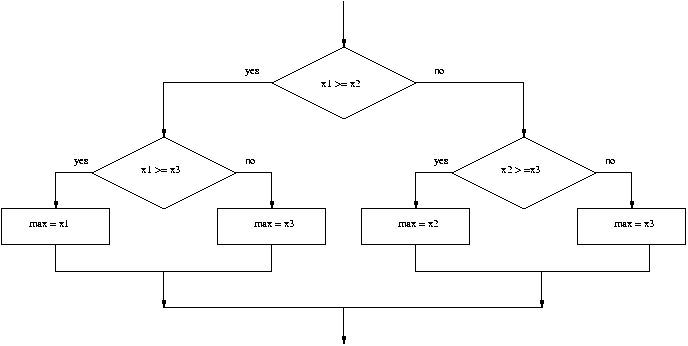
\includegraphics[width=11cm]{pic17}
\end{center}
\end{frame}

\begin{frame}[fragile]
  \frametitle{Strategija 2: stablo odlučivanja}
\begin{minted}[linenos=false]{python}
if x1 >= x2:
   if x1 >= x3:
      max = x1
   else:
      max = x3
else:
   if x2 >= x3:
      max = x2
   else
      max = x3
\end{minted}
\end{frame}

\begin{frame}[fragile]
  \frametitle{Strategija 2: stablo odlučivanja}
  \begin{itemize}
    \item sa ovim pristupom uvek imamo tačno 2 poređenja bez obzira na raspored brojeva
    \item komplikovanije od prve strategije:
    \item za traženje najvećeg od 4 broja trebaće nam \texttt{if-else} u tri nivoa, sa ukupno 8 naredbi dodele
  \end{itemize}
\end{frame}

\begin{frame}[fragile]
  \frametitle{Strategija 3: sekvencijalna obrada}
  \begin{itemize}
    \item šta ako dobijemo listu od 100 brojeva?
    \item idemo redom kroz listu i pamtimo najvećeg pronađenog do tog trenutka
    \item na kraju ćemo kao zapamćenog imati najveći broj
  \end{itemize}
\end{frame}

\begin{frame}[fragile]
  \frametitle{Strategija 3: sekvencijalna obrada}
\begin{center}
  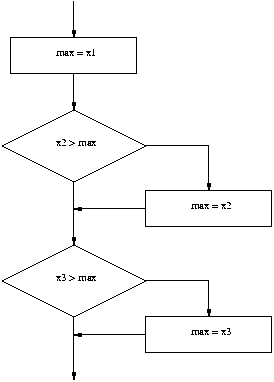
\includegraphics[width=5cm]{pic18}
\end{center}
\end{frame}

\begin{frame}[fragile]
  \frametitle{Strategija 3: sekvencijalna obrada}
  \begin{itemize}
    \item lako se prevodi u Python kod
  \end{itemize}
\begin{minted}[linenos=false]{python}
max = x1
if x2 > max:
    max = x2
if x3 > max:
    max = x3
\end{minted}
\end{frame}

\begin{frame}[fragile]
  \frametitle{Strategija 3: sekvencijalna obrada}
  \begin{itemize}
    \item ovaj postupak se ponavlja i lako se predstavlja petljom
    \item unesemo broj
    \item uporedimo ga sa trenutnim \texttt{max}
    \item ako je veći, ažuriramo \texttt{max}
    \item ponavljamo dok ima brojeva
  \end{itemize}
\end{frame}

\begin{frame}[fragile]
  \frametitle{Strategija 3: sekvencijalna obrada}
\begin{minted}[linenos=false]{python}
n = eval(raw_input("Koliko ima brojeva? "))

max = eval(raw_input("Unesite broj >> "))

for i in range(n-1): 
    x = eval(raw_input("Unesite broj >> "))
    if x > max:
        max = x

print "Najveći broj je", max
\end{minted}
\end{frame}

\begin{frame}[fragile]
  \frametitle{Strategija 4: koristi Python biblioteku}
  \begin{itemize}
    \item postoji funkcija \texttt{max} koja vraća najveći broj iz date liste
  \end{itemize}
\begin{minted}[linenos=false]{python}
x1, x2, x3 = eval(raw_input("Unesite tri broja: "))
print "Najveći broj je", max(x1, x2, x3)
\end{minted}
\end{frame}

\section{Moduli}

\begin{frame}[fragile]
  \frametitle{Python moduli}
  \begin{itemize}
    \item fajlovi sa Python kodom se mogu upotrebiti na više načina
    \item[1] neki su predviđeni da se direktno pokreću kao programi -- \myblue{programi} ili \myblue{skriptovi}
    \item[2] neki su predviđeni da se koriste kao \myblue{moduli}, tj. \texttt{import}-uju iz drugih programa
    \item[3] neki mogu da se koriste na oba načina
  \end{itemize}
\end{frame}

\begin{frame}[fragile]
  \frametitle{Python moduli $_2$}
  \begin{itemize}
    \item kako u nekom Python fajlu znamo da li smo pokrenuti direktno (kao program), ili \texttt{import}-ovani (kao modul)?
    \item najčešće kada \texttt{import}-ujemo modul, ne želimo da se on izvršava \\ \ \\
    \item u svakom Python fajlu možemo koristiti specijalnu promenljivu \texttt{\_\_name\_\_}
    \item u njoj je ime našeg modula (ako je fajl trenutno \texttt{import}-ovan)...
    \item ...ili je njena vrednost \texttt{"\_\_main\_\_"} ako je fajl pokrenut kao program
  \end{itemize}
\end{frame}

\begin{frame}[fragile]
  \frametitle{Python moduli $_3$}
\begin{minted}[linenos=false]{python}
# mojmodul.py

def fun1():
    ...

def fun2():
    ...

def main():
    ...

if __name__ == "__main__":
    main()
\end{minted}
\end{frame}

\begin{frame}[fragile]
  \frametitle{Python moduli $_4$}
\begin{minted}[linenos=false]{python}
if __name__ == "__main__":
    main()
\end{minted}
  \begin{itemize}
    \item ako smo ovaj fajl pokrenuli kao Python program: \\
    \texttt{\_\_name\_\_ == "\_\_main\_\_"}
    \item ako smo ovaj fajl \texttt{import}-ovali kao modul: \\
    \texttt{\_\_name\_\_ == "mojmodul"}
  \end{itemize}
\end{frame}

\end{document}